\section[德布罗意的“物质波”假设]{德布罗意的“物质波”假设}\label{sec:01.05}
% \makebox[5em][s]{} % 短题目拉间距
% \setlength{\mathindent}{9em} 本文标准公式缩进 
% \eqnormal % 恢复标准缩进

玻尔量子论的建立,极大地推动了原子物理学的发展.但随着研究的深入,玻尔量子论的局限性也逐渐暴露出来.例如任何一种原子光谱,各条谱线的相对强度表现出很好的规律性,玻尔量子论未能对此作出满意的解释.氨原子光谱表现出某些奇特的规律(似乎是由两套光谱混杂而成),玻尔量子论对此也无力解释长期以来,许多化学和物理理论中,从来认为原子的形状像一个小球,这个概念早已被多种实验事实所肯定. 但在玻尔量子论中,电子作平面轨道运动,因此原子(尤其是氢原子)的形状更像一个饼.

1924年,德布罗意提出了“物质波” 的假设.德布罗意注意到了几何光学(光的宏观传播规律)和质点力学有着惊人的相似性.光在均匀介质中沿直线传播的定律,在两种介质的分界面处光的反射和折射定律,以及在不均匀介质中光沿曲线传播的规律,可以统一为“最小光程原理(费马原理)”, 即
\eqshort
\begin{equation}\label{eq15.1}
	\delta\int_{A}^{B} ndl = 0
\end{equation}\eqnormal
光由A点传播到B点,$\int_{A}^{B}\cdots dl$表示由A到B的线积分,n为折射率,(A,B)间任何一条可能的路径的光程即$\int_{A}^{B}ndl$,光程最小的路径就是实际的光线.牛顿质点力学定律可以表示成“最小作用量原理”,即
\begin{equation}\label{eq15.2}
	\delta\int_{A}^{B}pdl=\delta\int_{A}^{B}\sqrt{2m(E\sim V)}dl
\end{equation}\eqlong
\begin{wrapfigure}[5]{r}{8em}
	\centering
	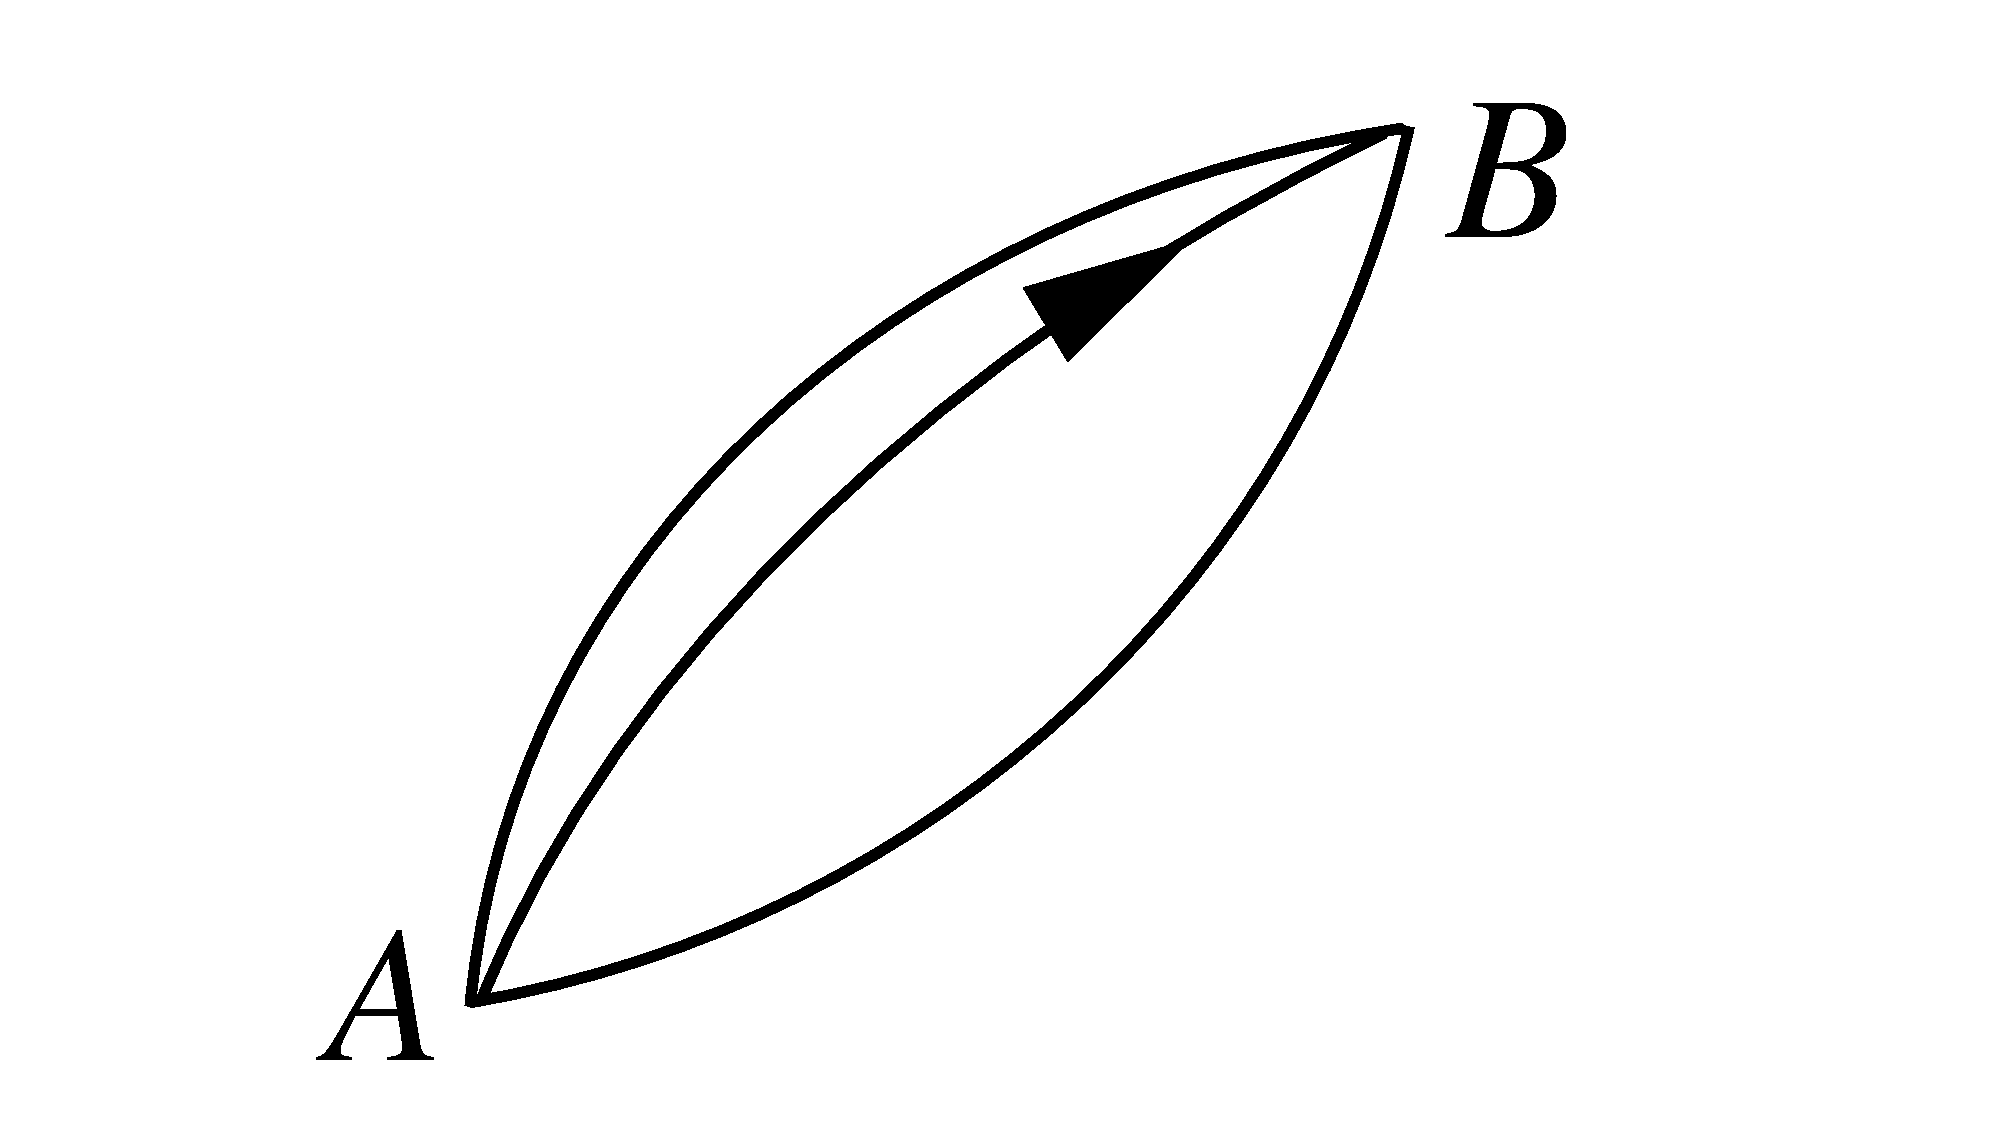
\includegraphics[width=2.5cm,clip]{QM file/figure/1-7}
	\caption{}
	\label{fig.1-7}
\end{wrapfigure}
其$m,p,E,V$表示质点的质量,动量,总能和势能,$\int pdl$称为作用量,质点由A至B的实际路径是作用量最小的路径.

德布罗意注意到光的本质包含者粒子和波动两个方面,光具有量子化的结构,每个光子具有一定的能量和动量:
\begin{equation}\label{eq15.3}
	E=\hbar\omega,\quad p=\frac{h}{\lambda},\quad \boldsymbol{p}=\hbar\boldsymbol{k}\quad
	(k=\frac{2\pi}{\lambda})
\end{equation}\eqnormal
在传播过程中,光表现出波动性,干涉、衍射等现象就是波动性的典型特征.但在宏观尺度上光的传播可以用光线概念来表述,波动光学表现为几何光学,波动规律以类似于力学规律的形式表现出来.德布罗意认为,电子以及其他物质粒子也都应该具有波动$\sim$粒子二重性.电子在结构上的量子性已为汤姆孙荷质比实验(测量$\frac{e}{m_{e}}$)所证实,电子在宏观尺度的运动遵守牛顿质点力学的规律,这早已被实验肯定.德布罗意认为,电子运动规律本质上应该是波动规律,这种波动性只有在微观尺度(量级和波长接近的尺度)才能表现出来,而在宏观尺度则表现为牛顿力学规律.德布罗意认为爱因斯坦公式\eqref{eq15.3}也适用于一切物质粒子,它们的力学性质$(E,p)$和波动性质$(\omega,\lambda)$通过普朗克常数$\hbar$互相联系.
\begin{wrapfigure}[8]{r}{8em}
	\centering
	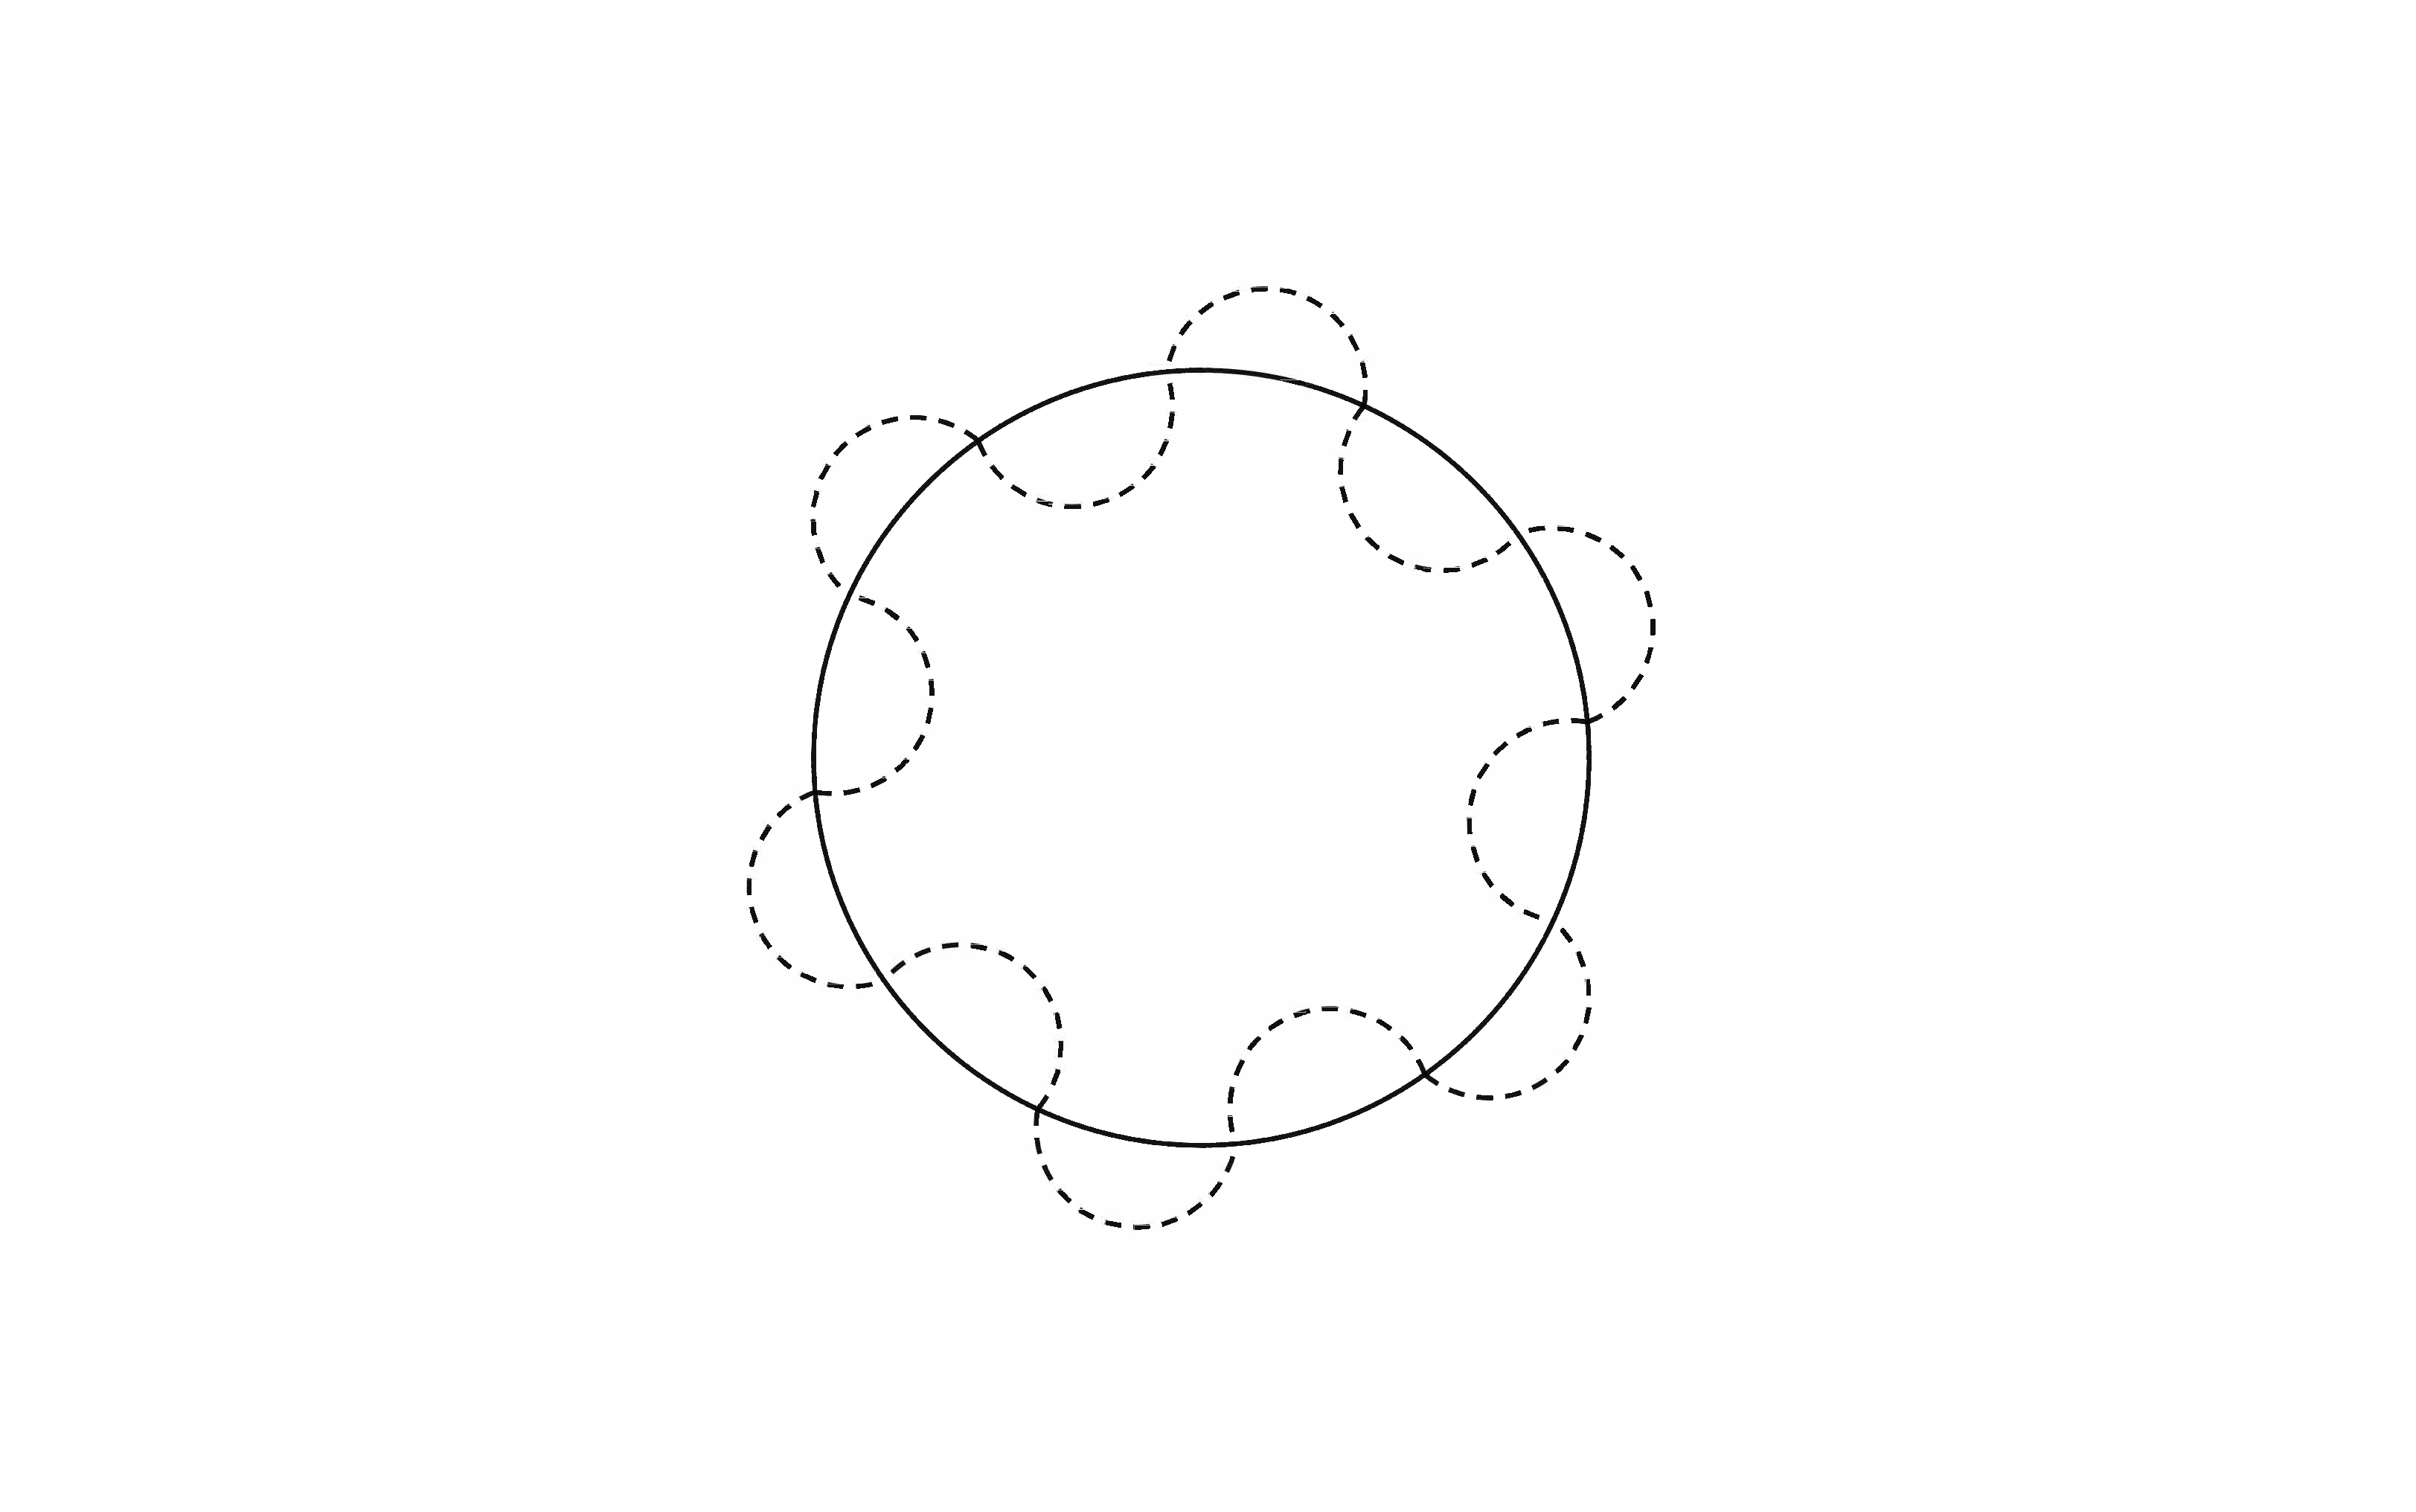
\includegraphics[width=2.5cm,clip]{QM file/figure/1-8}
	\caption{}
	\label{fig.1-8}
\end{wrapfigure}

德布罗意提出上述“物质波”设想时,并无直接的实验根据,而是一种科学假设.他希望这种未经证实的电子的波动性能够解释玻尔量子论所无法解释的那些困难问题.他指出,玻尔量子论中的量子化条件(这是玻尔理论中最难理解的一条)的实质很容易用波动的观点给以解释,如下.电子沿轨道运动,相当于物质波沿轨道传播,如果轨道周长不等于波长的整数倍,物质波将自行干涉而消失,亦即这种轨道是不允许的;如果轨道周长等于波长的整数倍,则物质波就能形成谐波而稳定存在,相应的轨道为稳定轨道形成谐波的条件为
\begin{equation}\label{eq15.4}
	\oint\frac{dq}{\lambda}=n,\quad n=1,2,3,\cdots	
\end{equation}
以$\lambda=\frac{h}{p}$代入上式,即得
\begin{equation}\label{eq15.5}
	\oint pdq=nh,\quad n=1,2,3,\cdots
\end{equation}
这正是量子化条件.

德布罗意的物质波思想直接导致了量子力学的诞生.相隔不到2年,薛定谔(E.Schr\"{o}dinger)就以“波动力学”的形式建立了量子力学(1926).稍早几个月,海森伯(W.Heisenberg)以“矩阵力学”的形式建立了量子力学(1925).

1927 年正式做了电子衍射实验,证实了电子确实具有波动性.接着又做了中子衍射实验,各种原子束和分子束的衍射实验,20世纪90年代还做了$C_{60}$分子(由60个碳原子形成的足球状大分子)束衍射实验,这些实验无一例外地都证实了公式$p=\frac{h}{\lambda}$的正确性,证实了实物粒子确实具有波动性.

当实物粒子在某种尺度的空间范围内运动时,如相应的物质波波长远小于空间尺度,一般可以不考虑粒子的波动性,而用经典力学处理粒子的运动.如波长接近或大于空间尺度,则波动性表现为粒子运动规律的主要方面,这时必须用量子力学来处理粒子的运动.下面举几个典型例子.

(1)气体分子的热运动.温度T下气体分子的热运动(平移)动能为$\frac{3kT}{2}$,$T=300 \si{K}$(室温)时,分子动能约为\num{0.039}\si{eV},相应的物质波波长为
\begin{equation*}
	\lambda=\frac{h}{p}=\frac{hc}{\sqrt{2m_{\text{分子}}\times\num{0.039}\si{eV}}}
\end{equation*}\eqshort
对于氧分子($O_{2}$),$m_{O_{2}}\approx32m_{p}\approx32\times938\times10^{6}\si{eV/c^{2}}$,波长$\lambda\approx0.026\si{nm}$,远小于分子的平均自由程,所以分子的热运动可作经典力学处理.

(2)原子中的电子运动电子动能的量级约10\si{eV},容易求得波长的量级为
\begin{equation*}
	\lambda\sim\frac{hc}{\sqrt{2m_{e}c^{2}E}}\sim 0.39\si{nm}
\end{equation*}\eqnormal
$\frac{\lambda}{2\pi}$和原子半径量级(0.1\si{nm})相同,所以要用量子力学来处理.

氢原子的基态,电子动能和动量为
\begin{equation*}
	\frac{p^{2}}{2m_{e}}=\frac{\e^{2}}{2a_{0}},\quad \boldsymbol{p}=\sqrt{\frac{m_{e}\e^{2}}{a_{0}}}=\frac{m_{e}\e^{2}}{\hbar}=\frac{\hbar}{a_{0}}
\end{equation*}\eqshort
波长为
\begin{equation*}
	\lambda=\frac{h}{p}=2\pi a_{0}
\end{equation*}\eqnormal
$a_{0}$为玻尔半径.

(3)原子核中核子的运动.核子(质子和中子)的动能约为$E\sim20 \si{MeV}$,相应的波长约为

\begin{equation}
	\begin{aligned}
		\lambda &\sim \frac{hc}{\sqrt{2m_{p}c^{2}E}}	\notag \\
				&\sim \frac{1.24\times10^{3} \si{MeV\cdot fm}}{\sqrt{2\times938\times20(\si{MeV})^{2}}}
				\approx 6.4 \si{fm}. \notag
	\end{aligned}
\end{equation}
核子的物质波波长$\lambda$和原子核半径同数量级,所以核子的运动也要用量子力学来处理.